%%%%%%%%%%%%%%%%%%%%%%%%%%%%%%%%%%%%%%%%%
% Election Computing System
% System obliczający i wizualizujący wyniki zgodnie z uogólnieniem systemu k-Borda na podstawie norm ell_p.
%
% Prezentacja wykonana na Pracownię Projektową
%
%%%%%%%%%%%%%%%%%%%%%%%%%%%%%%%%%%%%%%%%%

%----------------------------------------------------------------------------------------
%	PACKAGES AND THEMES
%----------------------------------------------------------------------------------------

\documentclass{beamer}

\usepackage[T1]{fontenc}
\usepackage[polish]{babel}
\usepackage[utf8]{inputenc}
\usepackage{lmodern}
\usepackage{amsmath}

\selectlanguage{polish}

\mode<presentation> {
	\usetheme{Copenhagen}
}

\usepackage{graphicx} % Allows including images
\usepackage{booktabs} % Allows the use of \toprule, \midrule and \bottomrule in tables
\usepackage{multicol} % columns
\usepackage{animate} % gif

% Custom macros

\newcommand{\red}[1]{
	{ \color{red}{#1} }
}

\newcommand{\score}[2]{
	\stackrel
	{\red{#1}}
	{#2}
}

\definecolor{links}{HTML}{2A1B81}
\hypersetup{colorlinks,linkcolor=,urlcolor=links}


%----------------------------------------------------------------------------------------
%	TITLE PAGE
%----------------------------------------------------------------------------------------

\title
[System obliczący wyniki wyborów]
{System obliczający wyniki wyborów dla uogólnienia systemu k-Borda}

\author
[T. Kasprzyk, D. Ogiela, J. Stępak]
{Tomasz Kasprzyk, \ Daniel Ogiela, \ Jakub Stępak}

\institute
[AGH]
{
Akademia Górniczo-Hutnicza

Wydział Informatyki, Elektroniki i Telekomunikacji

Katedra Informatyki 
\newline \newline
Projekt realizowany pod opieką \\dr. hab. inż. Piotra Faliszewskiego

}
\date{6 czerwca 2016}

%----------------------------------------------------------------------------------------

\begin{document}

\frame{\titlepage}

\begin{frame}
\frametitle{Plan}
\tableofcontents
\end{frame}

%----------------------------------------------------------------------------------------
%	PRESENTATION SLIDES
%----------------------------------------------------------------------------------------

%------------------------------------------------
\section{Rejestracja}
%------------------------------------------------
\subsection{Rejestracja}
%------------------------------------------------
\begin{frame}
\frametitle{Dane użytkownika}
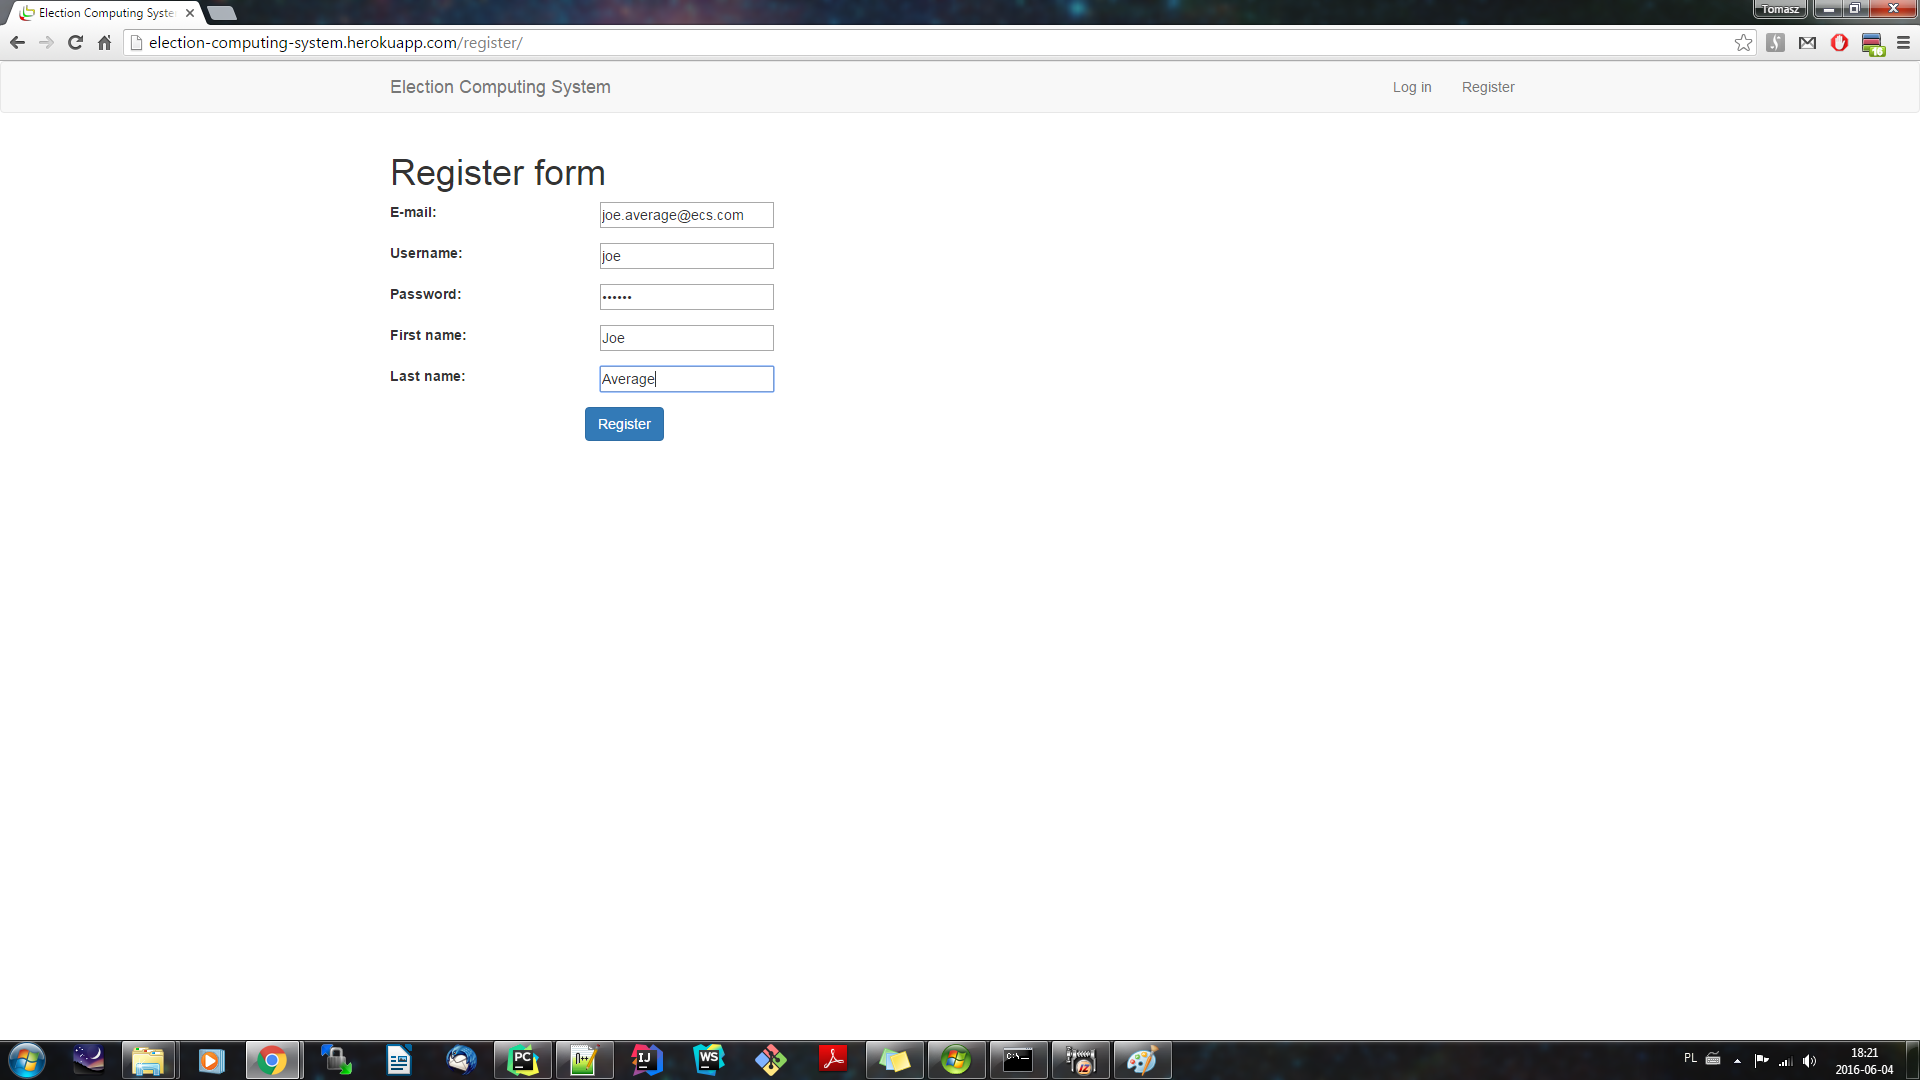
\includegraphics[height=0.63\paperheight]{screenshots/02_rejestracja.png}
\end{frame}
%------------------------------------------------
\begin{frame}
\frametitle{Uwierzytelnianie}
Django dostarcza w pełni funkcjonalny system uwierzytelniania. Zapewnia obsługę kont, grup oraz uprawnień użytkowników.
\end{frame}

%------------------------------------------------
\section{Tworzenie wyborów}
\begin{frame}
\frametitle{Panel dodawania wyborów}
\begin{center}
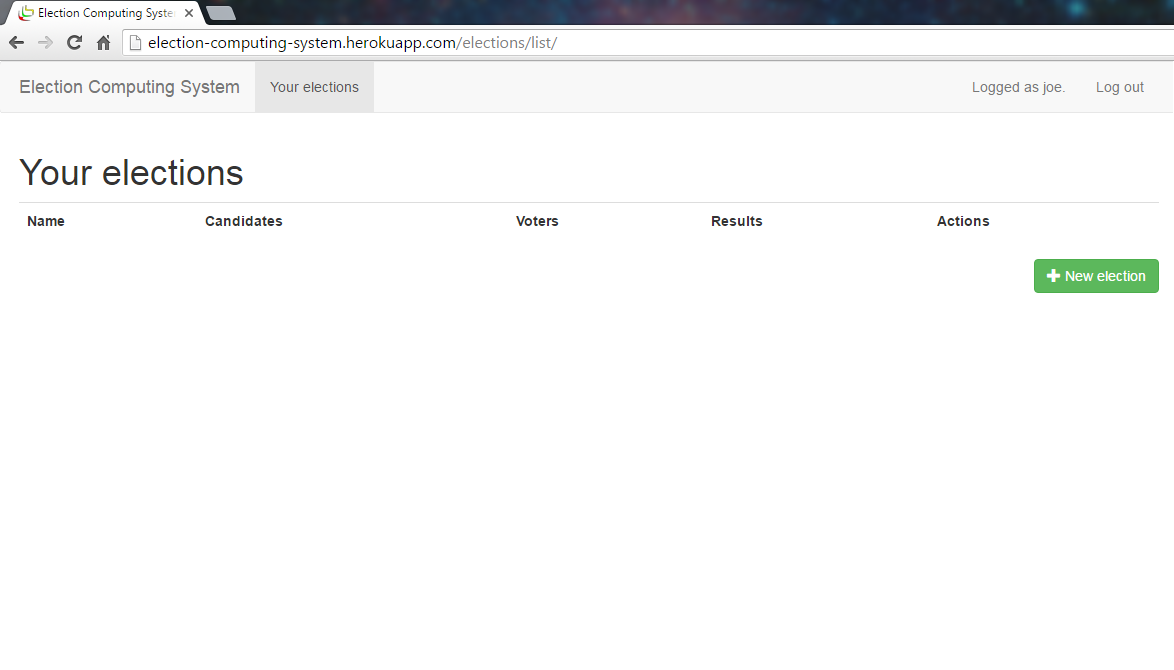
\includegraphics[width=0.8\paperwidth]{screenshots/04_new_elections.png}
\end{center}
\end{frame}
%------------------------------------------------
\begin{frame}
\frametitle{Dodawanie wyborów}
\begin{itemize}
	\item Z pliku
	\item Z rozkładu normalnego
	\item ?
\end{itemize}
\begin{center}
	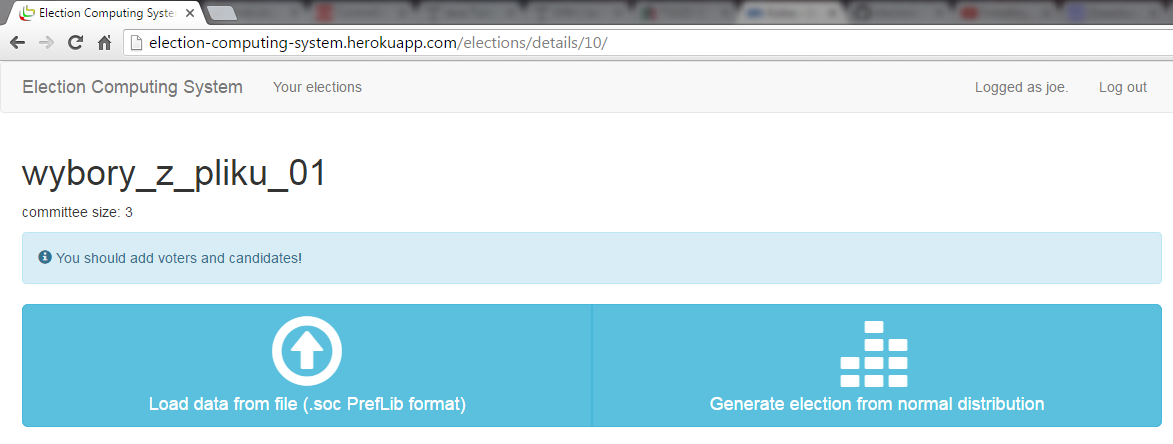
\includegraphics[width=0.8\paperwidth]{screenshots/06_add_election.png}
\end{center}
\end{frame}
%------------------------------------------------

\subsection{Pobieranie danych z pliku}
\begin{frame}
\frametitle{Pobieranie danych z pliku}
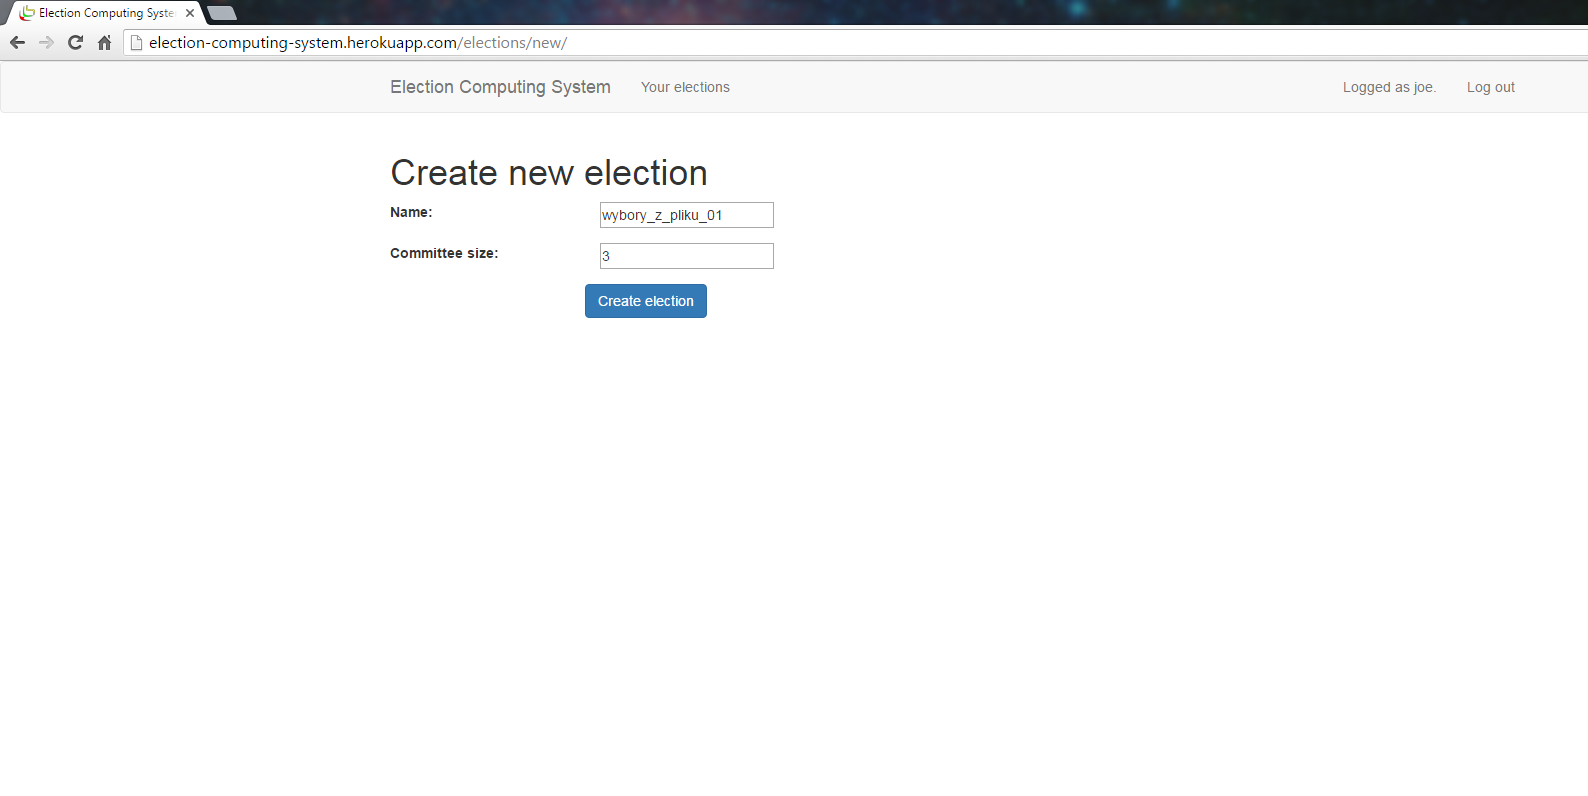
\includegraphics[width=0.8\paperwidth]{screenshots/05_file_elections_01.png}
\end{frame}


%------------------------------------------------
\begin{frame}
\frametitle{Dane gotowe do obliczania wyborów}
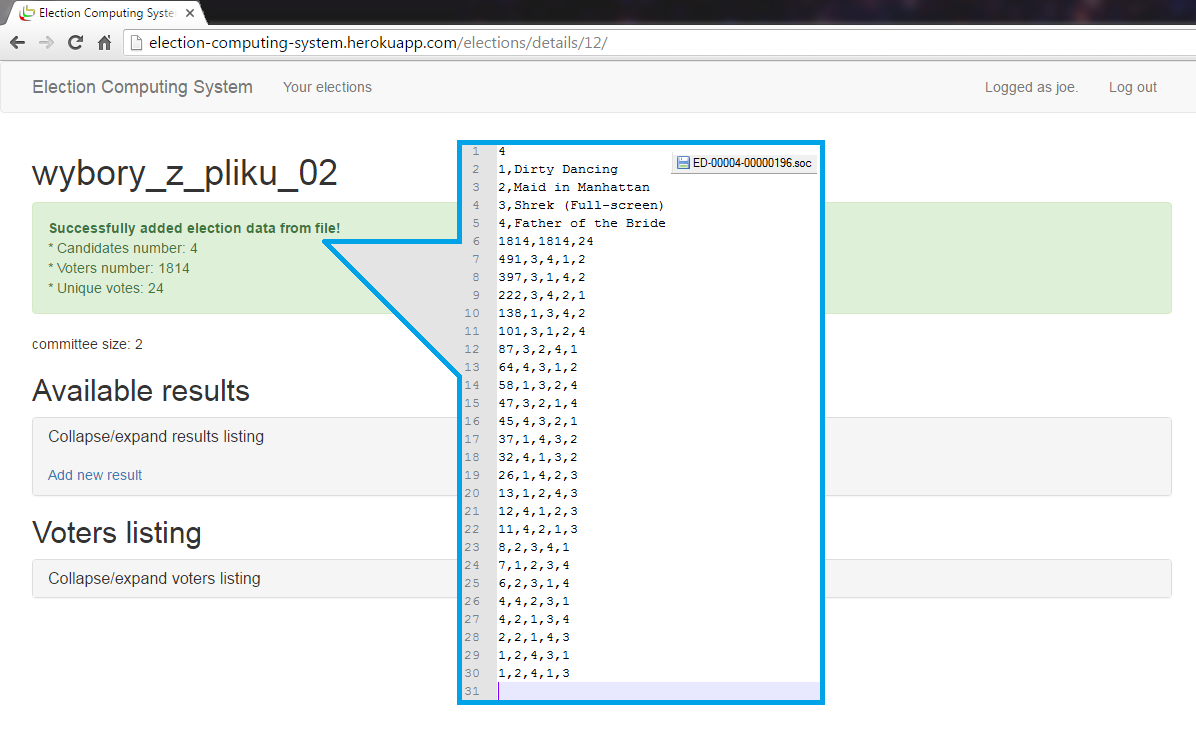
\includegraphics[width=0.8\paperwidth]{screenshots/10_soc_file_loaded_other.png}
\end{frame}

%------------------------------------------------
\subsection{Generowanie z rokładu normalnego}
\begin{frame}
\frametitle{Ustalanie parametrów populacji}
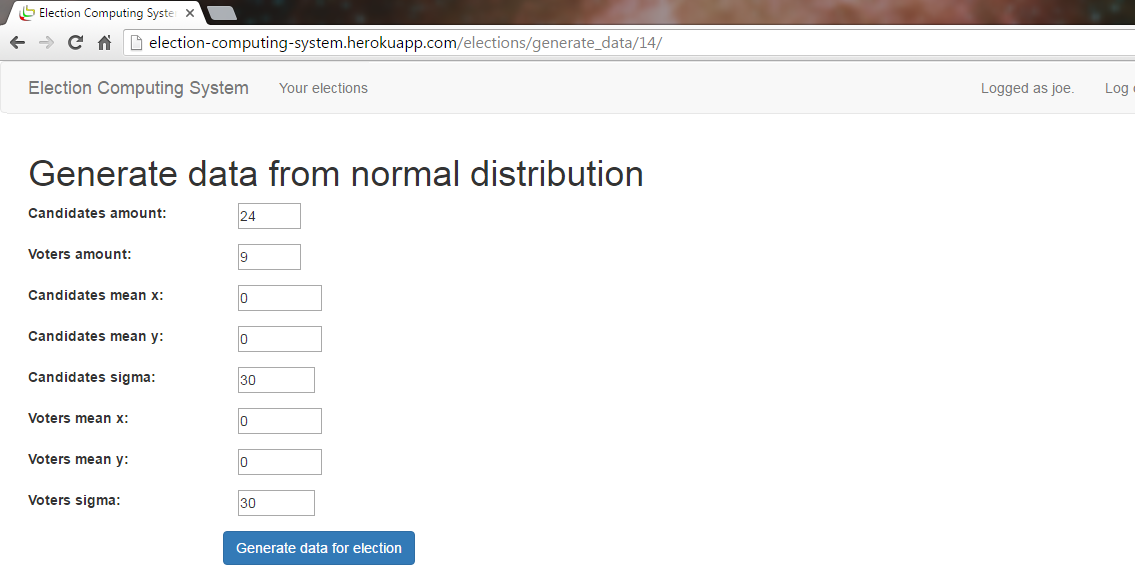
\includegraphics[width=0.8\paperwidth]{screenshots/16_normalny.png}
\end{frame}
%------------------------------------------------
\begin{frame}
\frametitle{Ustalanie parametrów populacji...}
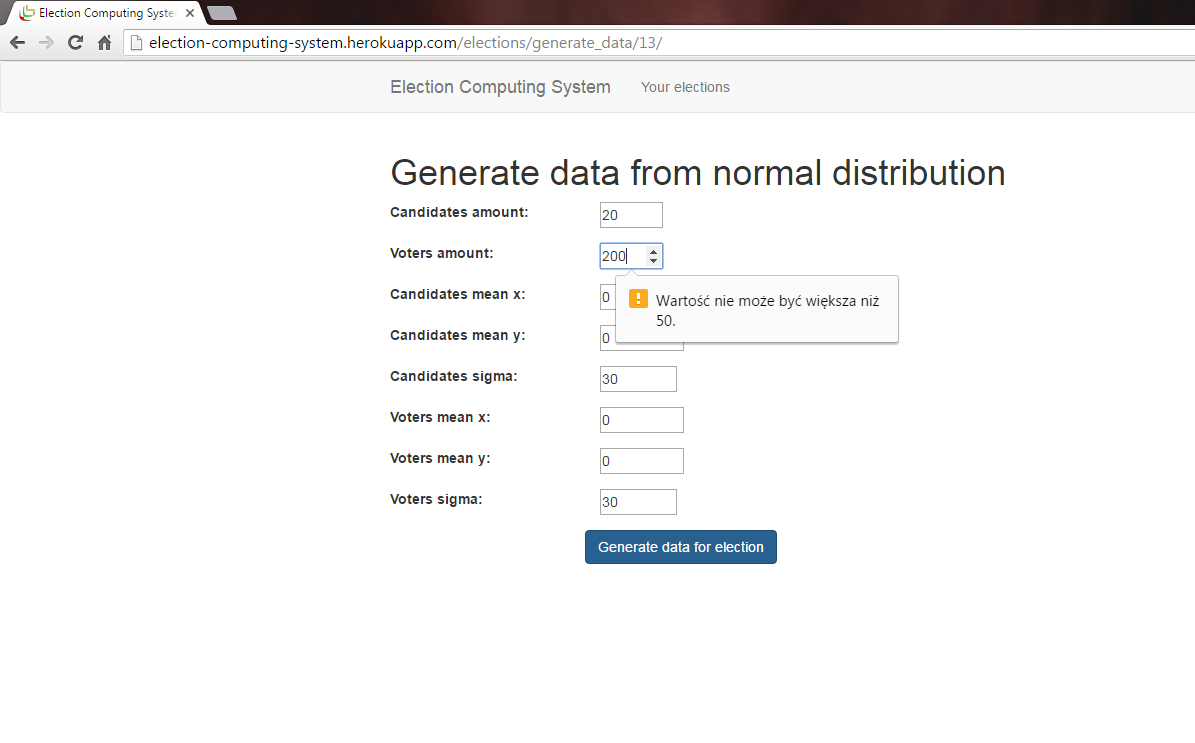
\includegraphics[height=0.5\paperheight]{screenshots/17_normalny_limit.png}
\begin{itemize}
\item ograniczenia na ilość wierszy w bazie danych
\item brak możliwości określenia timeoutu...
\end{itemize}
\end{frame}
%------------------------------------------------
\begin{frame}
\frametitle{Wykres}
\begin{multicols}{2}
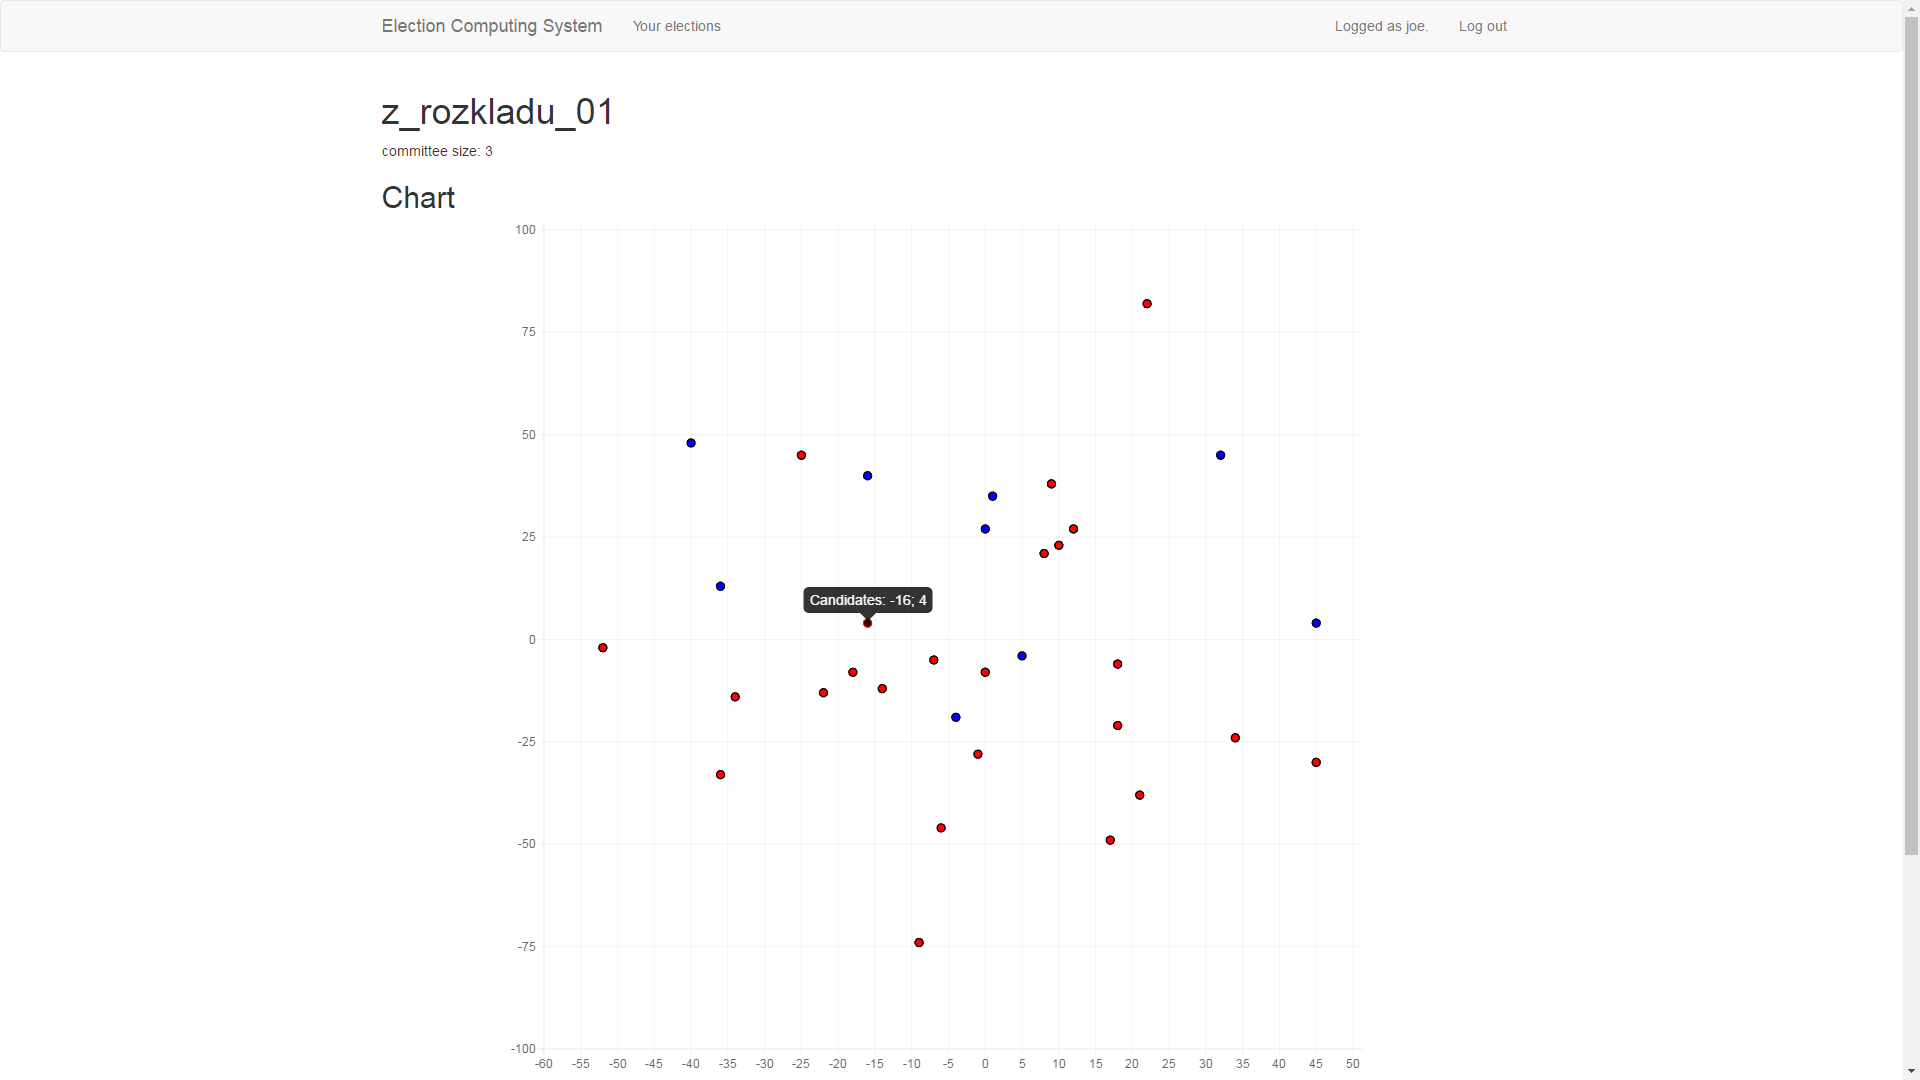
\includegraphics[height=0.6\paperheight]{screenshots/18_wykres.png}\\
Ulepszenie sposobu prezentacji
\begin{itemize}
\item dodatkowe informacje o punkcie
\item inne sposoby generowania wykresów...
\end{itemize}
\end{multicols}
\end{frame}
%------------------------------------------------
\begin{frame}
\frametitle{Lista preferencji}
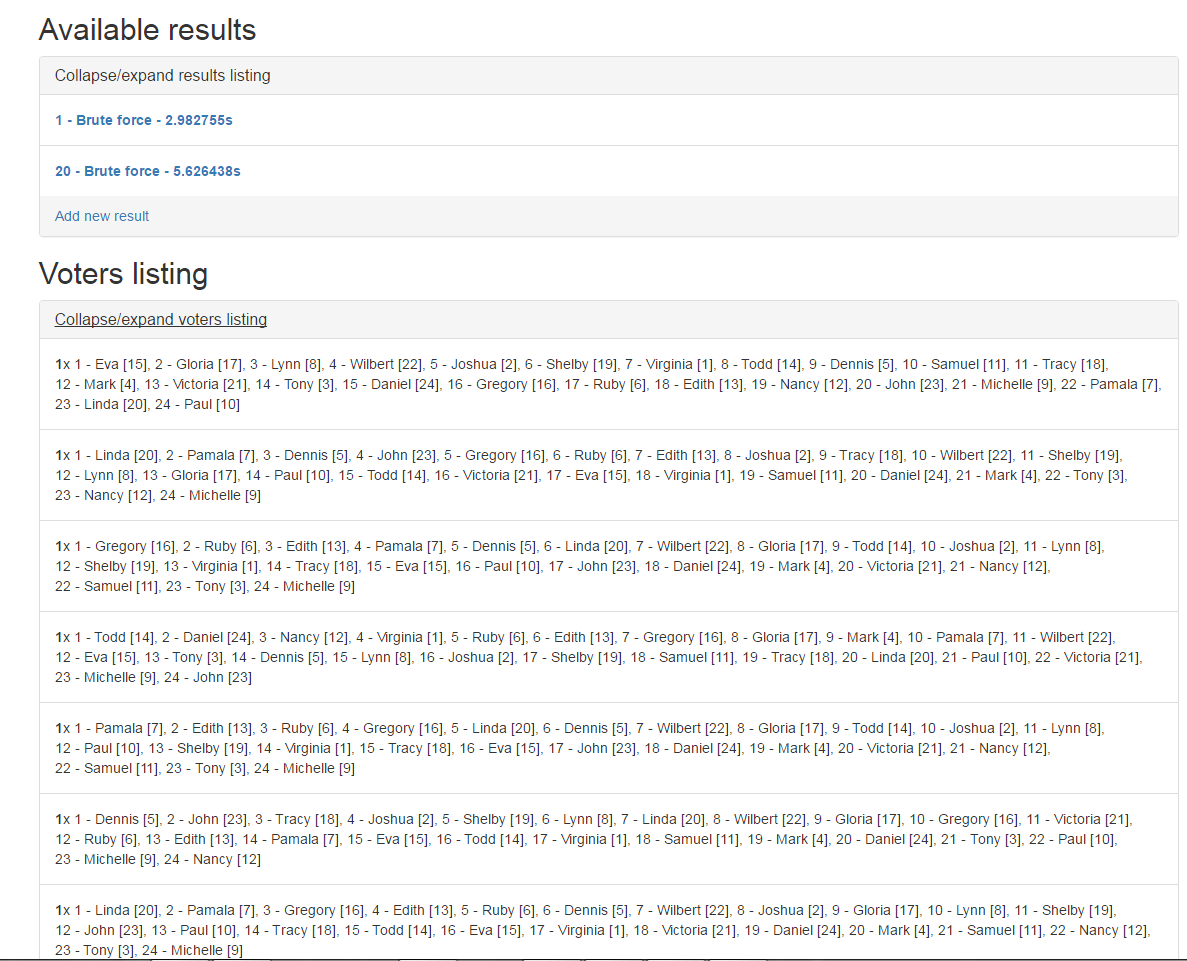
\includegraphics[height=0.5\paperheight]{screenshots/19_szczegoly.png}
\begin{itemize}
\item powiązanie danych z punktami
\end{itemize}
\end{frame}
%------------------------------------------------

\section{Obliczanie wyników}
\begin{frame}
\frametitle{Konfiguracja obliczeń}
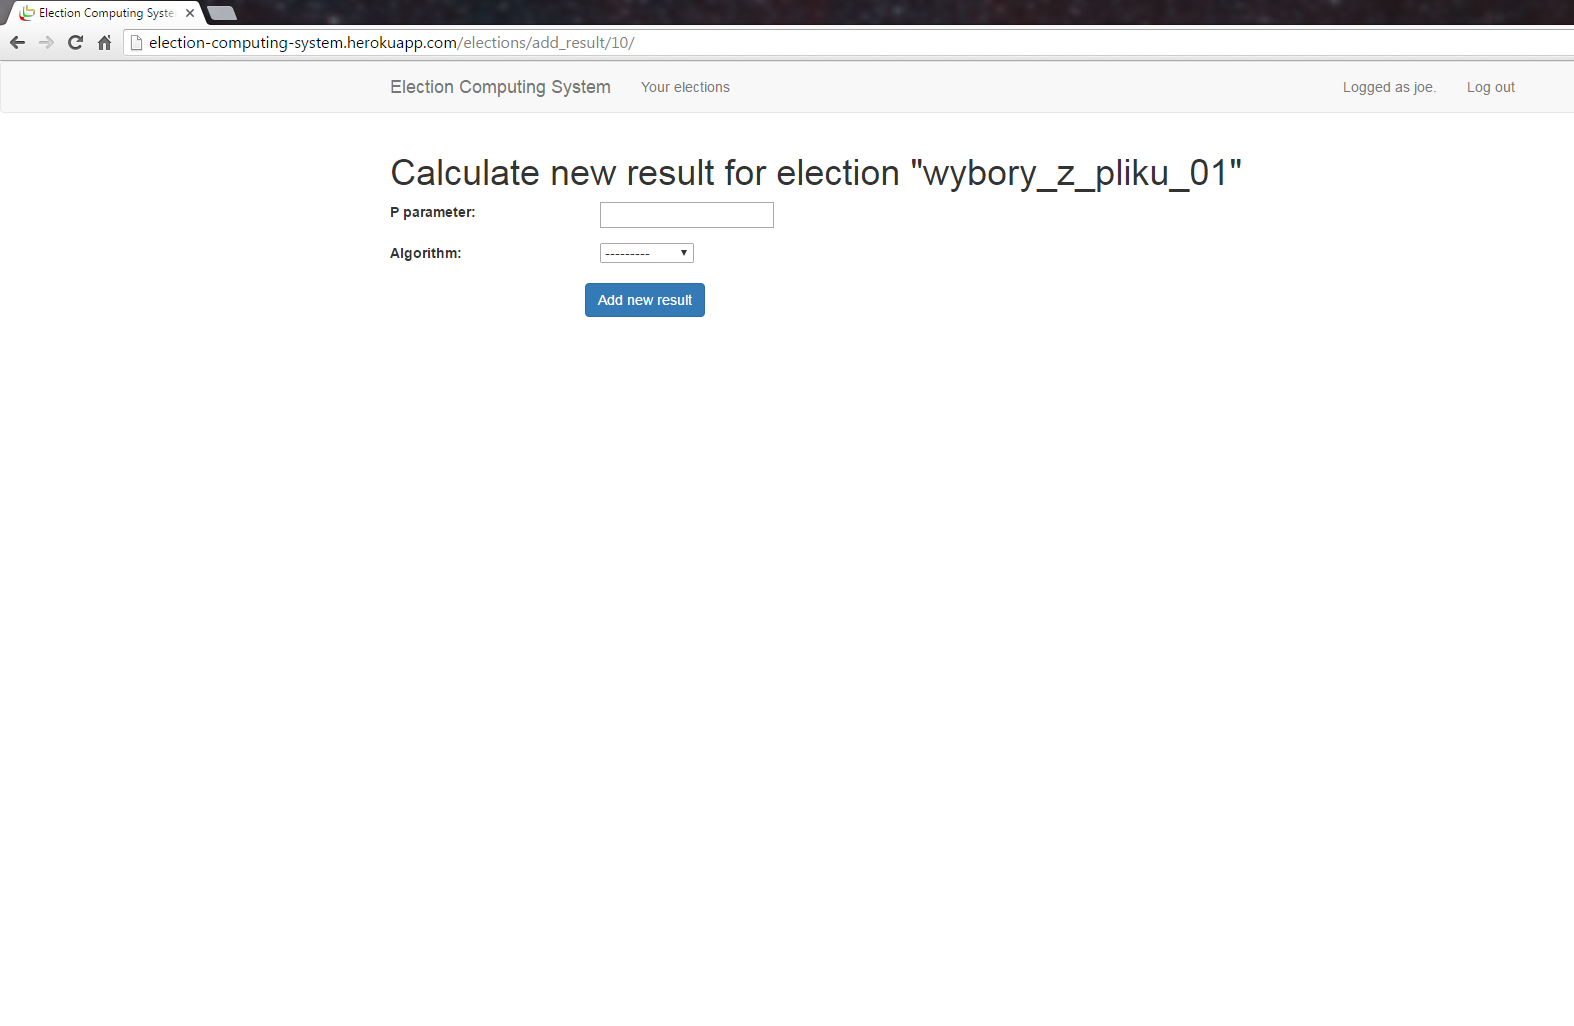
\includegraphics[width=0.8\paperwidth]{screenshots/12_add_new_result.png}
\begin{itemize}
\item możliwość wyboru algorytmu...
\item możliwość wyboru parametru
\end{itemize}
\end{frame}
%------------------------------------------------
\subsection{dla wyborów z pliku}
\begin{frame}
\frametitle{Rezultaty}
\begin{multicols}{2}
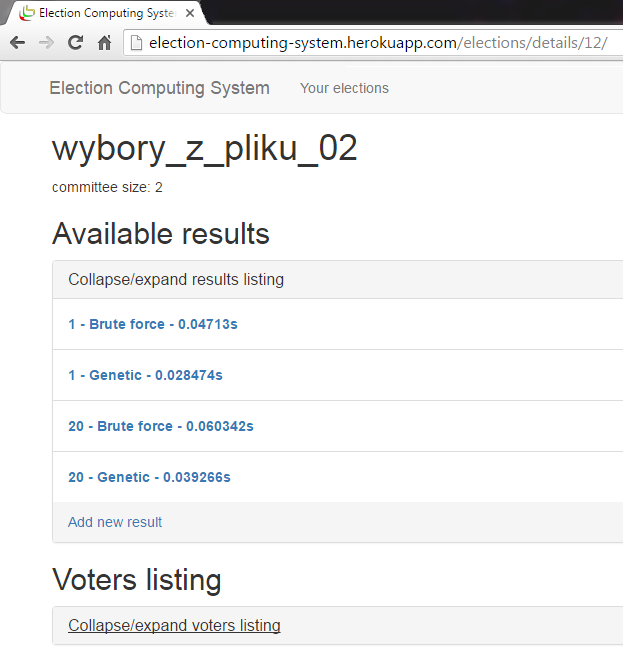
\includegraphics[height=0.5\paperheight]{screenshots/13_other_results.png}
\begin{itemize}
\item wybrany parametr p
\item zastosowany algorytm
\item czas wykonania obliczeń
\item wyniki wyborów pod linkiem
\end{itemize}
\end{multicols}
\end{frame}
%------------------------------------------------
\begin{frame}
\frametitle{Komitet}
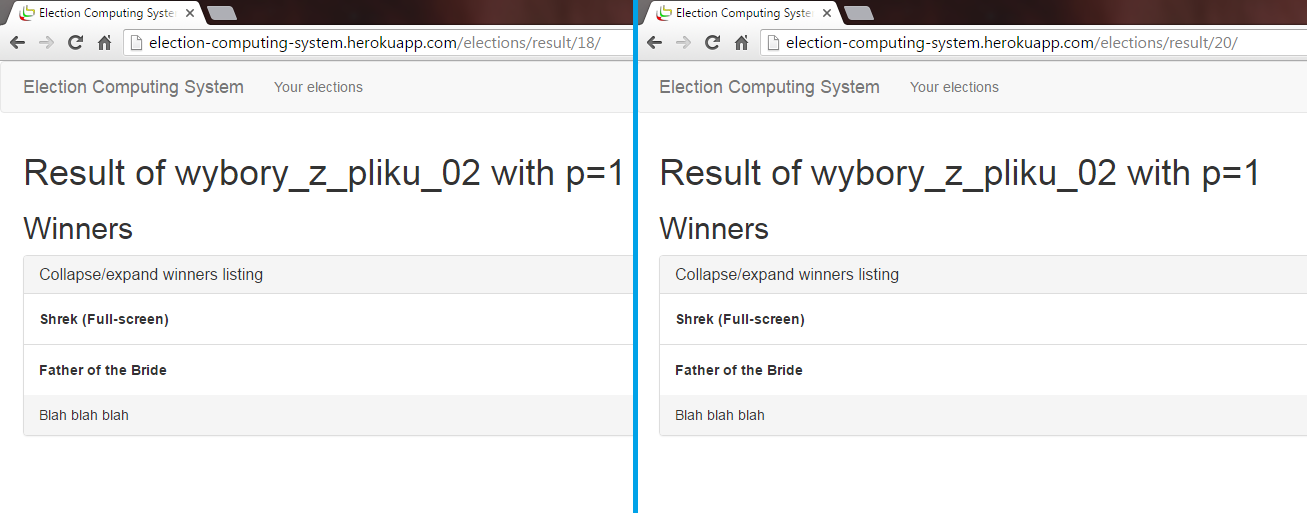
\includegraphics[width=0.8\paperwidth]{screenshots/15_genetic_brute_p1.png}
\end{frame}
%------------------------------------------------
\subsection{dla wyborów z rozkładu normalnego}
\begin{frame}
\frametitle{Rezultaty}
Wykres z zaznaczonymi zwycięzcami wyborów
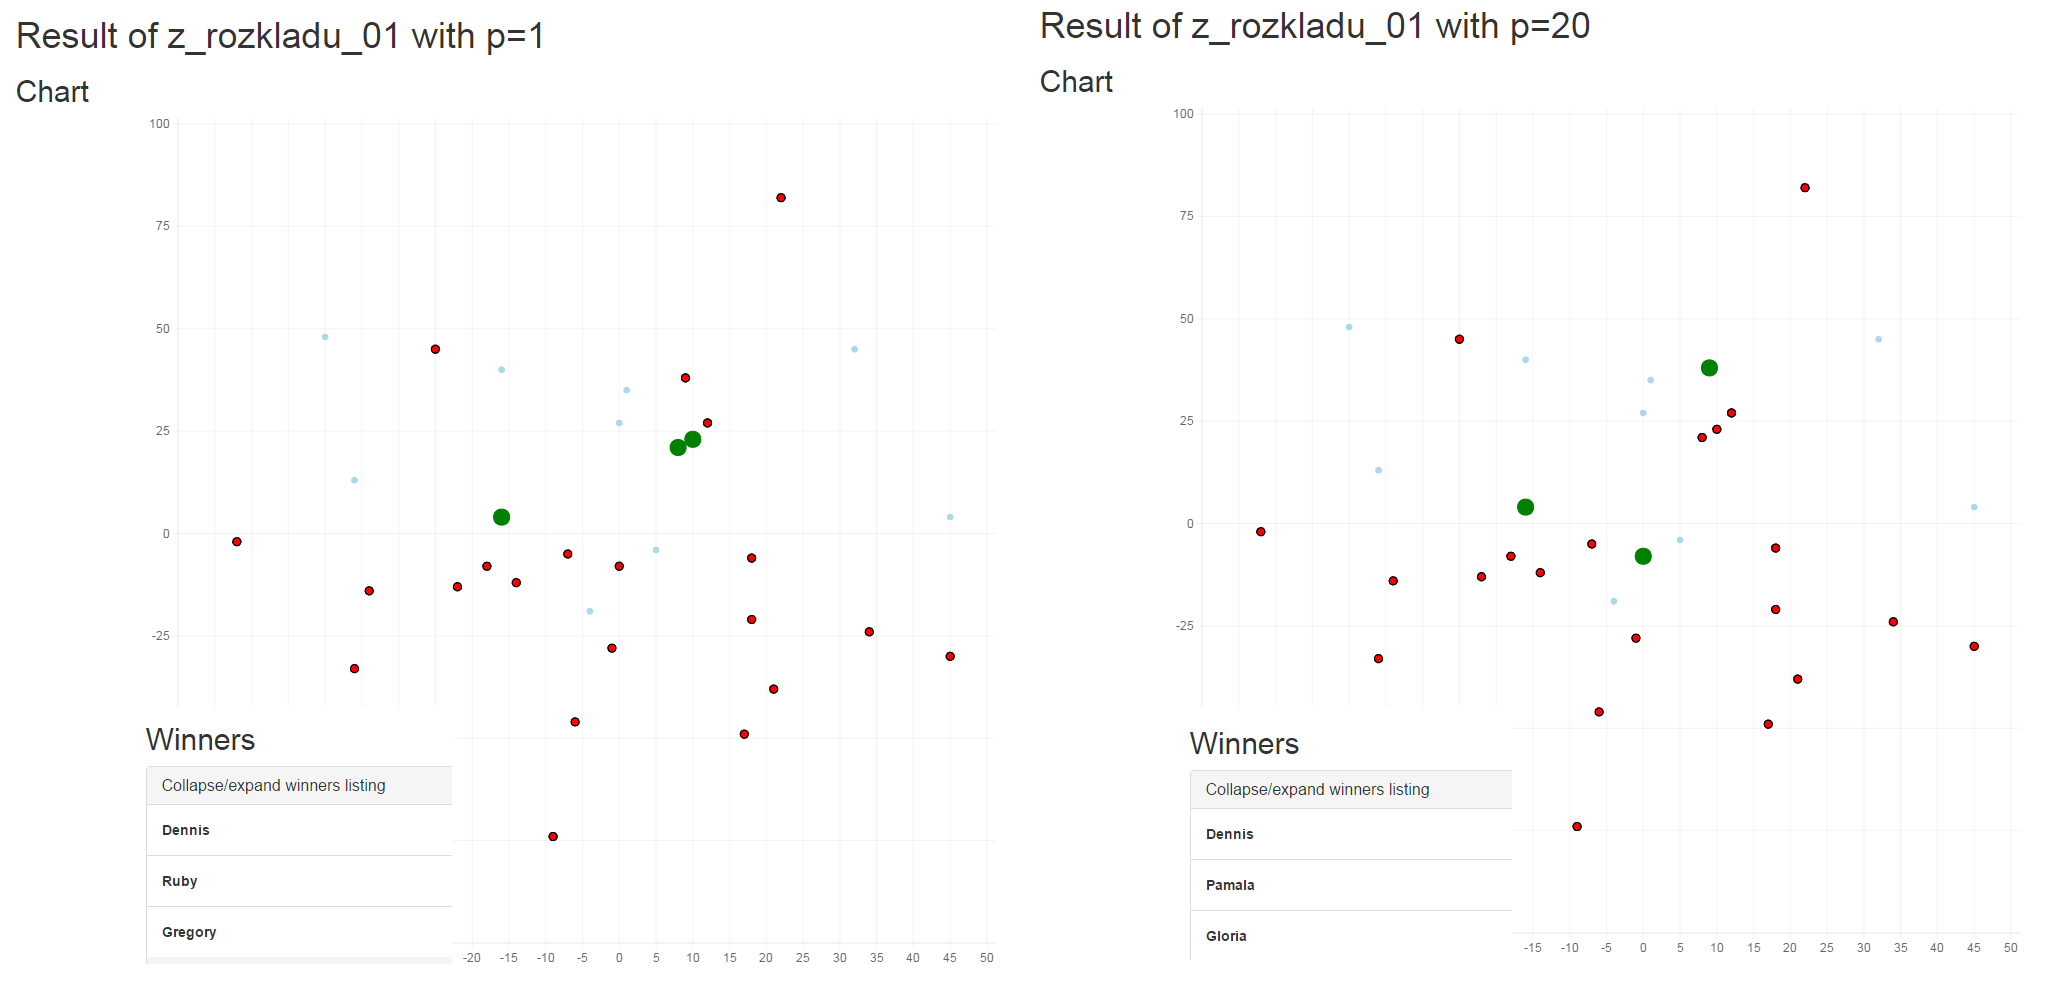
\includegraphics[width=0.8\paperwidth]{screenshots/20_brute_norm_1_20.png}
\end{frame}
%------------------------------------------------

\section{Usuwanie wyborów}
%------------------------------------------------
\subsection{usuwanie wyborów}
\begin{frame}
\frametitle{Usuwanie całych wyborów}
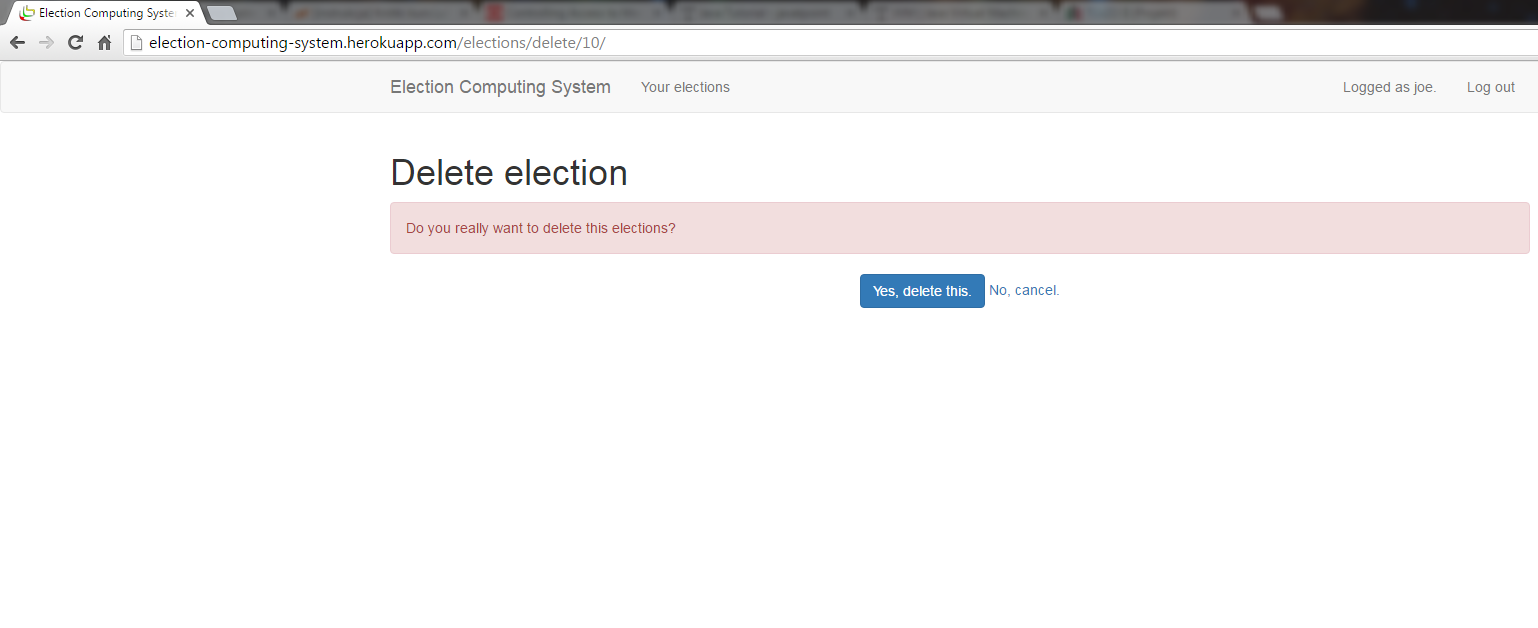
\includegraphics[width=0.8\paperwidth]{screenshots/21_delete.png}
\begin{itemize}
\item możliwość usuwania pojedynczych rezultatów w ramach wyborów
\end{itemize}
\end{frame}


\section{Podsumowanie}
%------------------------------------------------
\begin{frame}
\frametitle{Podsumowanie}
\begin{multicols}{2}
\begin{itemize}
\item implementacja wydajniejszych algorytmów
\item ulepszenie sposobu wyświetlania wyników
\item dodanie obliczania wyników wyborów w tle
\item możliwość malowania wykresów przez użytkownika
\item dynamiczna zmiana parametru p
\end{itemize}
\animategraphics[loop,autoplay, width=1\linewidth]{0.5}{screenshots/output/frame-}{0}{7}
\end{multicols}
\end{frame}
%------------------------------------------------

\begin{frame}
\Huge{\centerline{Dziękujemy za uwagę}}
\end{frame}

%----------------------------------------------------------------------------------------

\end{document} 
